\chapter{Свёрточные слои}
\label{chap:cnns}

\begin{supportbox}{Об этой главе}
В этой главе мы представляем наш второй основной слой, \textbf{свёрточный слой}, который предназначен для работы с изображениями (или, в более общем смысле, с последовательными данными любого рода), используя две ключевые идеи, которые мы называем \textit{локальностью} и \textit{разделением параметров}.
\end{supportbox}

Полносвязные слои важны с исторической точки зрения, но менее важны с практической: на неструктурированных данных (которые мы также называем \textbf{табличными} данными, поскольку их можно легко представить в виде таблицы) МЛП, как правило, уступают другим альтернативам, таким как случайные леса или хорошо настроенные машины опорных векторов \cite{grinsztajn2022tree}. Однако это не так, как только мы рассматриваем другие типы данных, имеющие некоторую структуру, которую можно использовать при проектировании слоев и модели.

В этой главе мы рассматриваем область изображений, в то время как в следующих главах мы также рассмотрим приложения к временным рядам, аудио, графам и видео. Во всех этих случаях вход имеет последовательную структуру (временную, пространственную или другого типа), которую можно использовать для проектирования слоев, которые являются одновременно производительными, легко компонуемыми и высокоэффективными с точки зрения параметров. Интересно, что мы увидим, что возможные решения можно спроектировать, взяв за отправную точку полносвязный слой, а затем соответствующим образом ограничив или обобщив его на основе свойств входа.
%
\section{На пути к свёрточным слоям}
\label{sec:towards_convolutive_layers}
%
\subsection{Почему полносвязных слоев недостаточно}
%
Изображение можно описать тензором $X \sim(h,w,c)$, где $h$ — высота изображения, $w$ — ширина изображения, а $c$ — количество каналов (которое может быть $1$ для черно-белых изображений, $3$ для цветных изображений или выше, например, для гиперспектральных изображений). Следовательно, мини-пакет изображений, как правило, будет иметь ранг $4$ с дополнительным ведущим измерением пакета $(b, h, w, c)$. Три измерения не идентичны, поскольку $h$ и $w$ представляют пространственное расположение \textit{пикселей}, в то время как каналы $c$ не имеют определенного порядка, в том смысле, что хранение изображений в формате RGB или GBR — это всего лишь вопрос соглашения. 

\begin{supportbox}{О нотации, каналах и признаках}
Мы используем тот же символ, который мы использовали для признаков в табличном случае ($c$), потому что он будет играть аналогичную роль в проектировании моделей, т.е. мы можем думать о каждом пикселе как об описанном общим набором из $c$ \textit{признаков}, которые обновляются параллельно слоями модели. Следовательно, свёрточный слой вернет общий тензор $(h,w,c^\prime)$ с вложением размера $c^\prime$ для каждого из $hw$ пикселей.
\end{supportbox}

Чтобы использовать полносвязный слой, нам нужно было бы «сплющить» (векторизовать) изображение:
%
\begin{equation}
\mathbf{h} =\phi(\mathbf{W}\cdot \eqnmarkbox[drawred]{node}{\text{vect}(X)})
\label{eq:basic_image_layer}
\end{equation}
\annotate[yshift=-1em]{below,right}{node}{Сплющенное изображение}

\vspace{1em}
где $\text{vect}(x)$ эквивалентно {\footnotesize\mintinline{python}{x.reshape(-1)}} в PyTorch, и для общего тензора ранга $n$ $x \sim (i_1, i_2, \ldots, i_n)$ возвращает эквивалентный тензор $\mathbf{x} \sim \left(\prod_{j=1}^n i_j\right)$.


Хотя должно быть ясно, что это неэлегантный подход, стоит подчеркнуть некоторые его недостатки. Во-первых, мы потеряли очень важное свойство из предыдущего раздела, а именно, \textbf{компонуемость}: наш вход — это изображение, а наш выход — вектор, что означает, что мы не можем объединить два таких слоя. Мы можем восстановить это, изменив форму выходного вектора на изображение:
%
\begin{equation}
H = \text{unvect}(\phi(\mathbf{W}\cdot\text{vect}(X)))
\end{equation}
%
где мы предполагаем, что слой не изменяет количество пикселей, и $\text{unvect}$ изменяет форму выхода на тензор $(h,w,c^\prime)$, где $c^\prime$ — гиперпараметр. 

Это напрямую ведет ко второй проблеме, которая заключается в том, что слой имеет \textit{огромное} количество параметров. Рассматривая, например, изображение RGB размером (1024, 1024), сохранение той же размерности на выходе приводит к $(1024*1024*3)^2$ параметрам (или $(hw)^2cc^\prime)$ в общем), что составляет порядка $10^{13}$! Мы можем интерпретировать предыдущий слой следующим образом: для каждого пикселя каждый канал на выходе является взвешенной комбинацией \textit{всех} каналов \textit{всех} пикселей на входном изображении. Как мы увидим, мы можем получить более эффективное решение, ограничив это вычисление.

\begin{supportbox}{Подробнее об изменении формы}
%
Чтобы сплющить (или, в более общем смысле, изменить форму) тензор, нам нужно определить порядок, в котором обрабатывать значения. На практике это определяется тем, как тензоры хранятся в памяти: в большинстве фреймворков данные тензора хранятся последовательно в непрерывном блоке памяти, в так называемом \textbf{шаговом расположении}. Рассмотрим следующий пример:

\vspace{1em}
\begin{center}
\footnotesize
\mintinline{python}{torch.randn(32, 32, 3).stride() # [Out]: (96, 3, 1)}
\end{center}
\vspace{1em}

Шаг — это количество шагов, которые необходимо сделать в памяти, чтобы переместиться на $1$ позицию вдоль этой оси, т.е. последнее измерение тензора является непрерывным, в то время как для перемещения на одну позицию в первом измерении нам нужно $96$ ($32*3$) шагов. Это называется \textbf{построчным} порядком или, в анализе изображений, \textbf{растровым} порядком.\footnote{\url{https://en.wikipedia.org/wiki/Raster_scan}} Каждая операция изменения формы работает путем перемещения по этому шаговому представлению.
%
\end{supportbox}

В качестве текущего примера для визуализации того, что следует, рассмотрим 1D-последовательность (мы рассмотрим 1D-последовательности более подробно позже; пока вы можете думать об этом как о «\textit{4 пикселях с одним каналом}»):

$$
\mathbf{x} = \left[x_1, x_2, x_3, x_4\right]
$$
%
В этом случае нам не нужны никакие операции изменения формы, и предыдущий слой (с $c^\prime = 1$) можно записать как:
%
$$
\begin{bmatrix} h_1 \\ h_2 \\ h_3 \\ h_4 \end{bmatrix}=\begin{bmatrix}W_{11} & W_{12} & W_{13} & W_{14} \\ W_{21} & W_{22} & W_{23} & W_{24} \\ W_{31} & W_{32} & W_{33} & W_{34} \\ W_{41} & W_{42} & W_{43} & W_{44} \end{bmatrix} \begin{bmatrix} x_1 \\ x_2 \\ x_3 \\ x_4 \end{bmatrix}
$$

\begin{SCfigure}
    \centering
    \hspace{1em}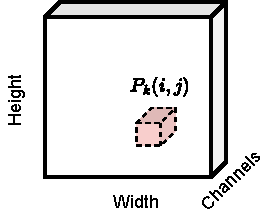
\includegraphics[width=0.4\textwidth]{images/patch}
    \caption{Для тензора $(h,w,c)$ и максимального расстояния $k$, \textbf{патч} $P_k(i,j)$ (показан красным) — это тензор $(2k+1,2k+1,c)$, собирающий все пиксели на расстоянии не более $k$ от пикселя в позиции $(i,j)$.}
    \label{fig:patch}
\end{SCfigure}

\subsection{Локальные слои}

Пространственное расположение пикселей вводит метрику (расстояние) между пикселями. Хотя существует много допустимых понятий «расстояния», нам будет удобно работать со следующим определением, которое определяет расстояние между пикселями $(i,j)$ и $(i^\prime, j^\prime)$ как максимальное расстояние по двум осям:
%
\begin{equation}
d((i,j), (i^\prime,j^\prime))=\max(\lvert i-i^\prime \rvert,\lvert j-j^\prime\rvert)
\label{eq:pixel_distance}
%
\end{equation}

Как мы можем использовать эту идею в определении слоя? В идеале мы можем представить, что влияние одного пикселя на другой уменьшается с коэффициентом, обратно пропорциональным их расстоянию. Доводя эту идею до крайности, мы можем предположить, что влияние фактически равно нулю для расстояния, превышающего некоторый порог. Чтобы формализовать это понимание, мы вводим понятие \textbf{патча}.

\begin{definition}[Патч изображения] \addbottle
Для изображения $X$, мы определяем \textbf{патч} $P_{k}(i,j)$ как подизображение с центром в $(i,j)$ и содержащее все пиксели на расстоянии, равном или меньшем $k$:
%
$$
P_{k}(i,j) = \idx{X}{i-k:i+k,j-k:j+k,:}
$$
%
где расстояние определяется как в \eqref{eq:pixel_distance}. Это визуально показано на Рисунке \ref{fig:patch}.
%
\end{definition}



Определение справедливо только для пикселей, которые находятся на расстоянии не менее $k$ шагов от границ изображения: мы пока проигнорируем этот момент и вернемся к нему позже. Каждый патч имеет форму $(s,s,c)$, где $s=2k+1$, поскольку мы рассматриваем $k$ пикселей в каждом направлении вместе с центральным пикселем. По причинам, которые будут разъяснены позже, мы называем $s$ \textbf{размером фильтра} или \textbf{размером ядра}.

Рассмотрим общий слой $H = f(X)$, принимающий на вход тензор формы $(h,w,c)$ и возвращающий тензор формы $(h,w,c^\prime)$. Если выход для данного пикселя зависит только от патча предопределенного размера, мы говорим, что слой \textbf{локальный}.

\begin{definition}[Локальный слой]
Для входного изображения $X \sim(h,w,c)$ слой $f(X) \sim(h,w,c^\prime)$ является \textbf{локальным}, если существует $k$ такое, что:
%
$$
\idx{f(X)}{ij} = f(P_{k}(i, j))
$$
%
Это должно выполняться для всех пикселей изображения.
%
\end{definition}

Мы можем преобразовать слой \eqref{eq:basic_image_layer} в локальный слой, установив в $0$ все веса, принадлежащие пикселям за пределами области влияния (\textbf{рецептивного поля}) каждого пикселя:

\vspace{1em}
$$
H_{ij} =\phi\left(\eqnmarkbox[drawgreen]{node2}{\mathbf{W}_{ij}}\cdot\eqnmarkbox[drawred]{node}{\text{vect}(P_{k}(i,j))}\right)
$$
\annotate[yshift=1em]{above,right}{node}{Сплющенный патч (формы $s^2c^\prime c$)}
\annotate[yshift=-1em]{below,right}{node2}{Зависящая от позиции весовая матрица}

\vspace{1em}
Мы называем этот класс слоев \textbf{локально-связными}. Обратите внимание, что у нас есть разная весовая матрица $\mathbf{W}_{ij} \sim({c^\prime, ssc})$ для каждого выходного пикселя, что приводит к $hw(s^2cc^\prime)$ параметрам. Для сравнения, в начальном слое у нас было $(hw)^2cc^\prime$ параметров, что дает коэффициент уменьшения $\frac{s^2}{hw}$ в количестве параметров.

Рассматривая наш игрушечный пример, предполагая, например, $k=1$ (следовательно, $s=3$), мы можем записать результирующую операцию как:
%
$$
\begin{bmatrix} h_1 \\ h_2 \\ h_3 \\ h_4 \end{bmatrix}=\begin{bmatrix}W_{12} & W_{13} & {\color{drawred}0} & {\color{drawred}0} \\ W_{21} & W_{22} & W_{23} & {\color{drawred}0} \\ {\color{drawred}0} & W_{31} & W_{32} & W_{33} \\ {\color{drawred}0} & {\color{drawred}0} & W_{41} & W_{42} \end{bmatrix} \begin{bmatrix} x_1 \\ x_2 \\ x_3 \\ x_4 \end{bmatrix}
$$
%
Наша операция не определена для $x_1$ и $x_4$, и в этом случае мы рассмотрели «укороченный» фильтр, удалив веса, соответствующие неопределенным операциям. Эквивалентно, вы можете думать о добавлении $0$ на границе, когда это необходимо:
%
$$
\begin{bmatrix} h_1 \\ h_2 \\ h_3 \\ h_4 \end{bmatrix}=\begin{bmatrix}W_{11} & W_{12} & W_{13} & 0 & 0 & {\color{drawred}0}\\ {\color{drawred}0} & W_{21} & W_{22} & W_{23} & 0 & {\color{drawred}0}\\ {\color{drawred}0} & 0 & W_{31} & W_{32} & W_{33} & {\color{drawred}0} \\ {\color{drawred}0} & 0 & 0 & W_{41} & W_{42} & W_{43} \end{bmatrix} \begin{bmatrix} {\color{drawred}0} \\ x_1 \\ x_2 \\ x_3 \\ x_4 \\ {\color{drawred}0} \end{bmatrix}
$$
%
Эта техника называется \textbf{дополнением нулями}. На изображении для размера ядра $2k+1$ нам нужно ровно $k$ строк и столбцов из $0$ с каждой стороны, чтобы гарантировать, что операция действительна для каждого пикселя. В противном случае выход не может быть вычислен вблизи границ, и выходной тензор будет иметь форму $(h-2k, w-2k, c^\prime)$. Оба варианта являются допустимыми в большинстве фреймворков.

\begin{supportbox}{О нашем определении патчей}
Определение свёрток с использованием идеи патчей немного нетрадиционно, но я нахожу, что оно значительно упрощает нотацию. Позже я приведу более традиционное, ориентированное на обработку сигналов определение. Эти два определения эквивалентны и могут использоваться взаимозаменяемо. Определение, ориентированное на патчи, требует \textbf{нечетного} размера ядра и не допускает \textbf{четных} размеров ядра, но последние на практике встречаются редко.
\end{supportbox}

\subsection{Трансляционная эквивариантность и свёрточный слой}

\addclock В локально-связном слое два идентичных патча могут приводить к разным выходам в зависимости от их местоположения: некоторое содержимое на пикселе $(5,2)$, например, будет обработано иначе, чем то же содержимое на пикселе $(39, 81)$, потому что две матрицы $\mathbf{W}_{5,2}$ и $\mathbf{W}_{39,81}$ различны. Однако по большей части мы можем предположить, что эта информация не имеет значения: неформально, «лошадь — это лошадь», независимо от ее положения на входном изображении. Мы можем формализовать это свойством, называемым \textbf{трансляционной эквивариантностью}.

\begin{definition}[Трансляционная эквивариантность]
Мы говорим, что слой $H = f(X)$ является \textbf{трансляционно эквивариантным}, если:

$$
\eqnmarkbox[drawred]{node}{P_{k}(i,j) = P_{k}(i^\prime, j^\prime)} \;\; \textnormal{подразумевает} \;\;  \eqnmarkbox[drawgreen]{node2}{f(P_{k}(i,j)) = f(P_{k}(i^\prime, j^\prime))}
$$
\annotate[yshift=-1em]{below,left}{node}{Идентичные патчи}
\annotate[yshift=-1em]{below,right}{node2}{Идентичные выходы}

\end{definition}

\vspace{0.5em}
Чтобы понять номенклатуру, обратите внимание, что мы можем интерпретировать предыдущее определение следующим образом: всякий раз, когда объект перемещается (транслируется) на изображении из положения $(i,j)$ в положение $(i^\prime, j^\prime)$, выход $f(P_{k}(i,j))$, который мы имели в $(i,j)$, теперь будет найден в $f(P_{k}(i^\prime,j^\prime))$. Следовательно, активации слоя движутся с тем же (\textit{èqui} на латыни) трансляционным движением, что и вход. Мы определим более формально эквивариантность и инвариантность позже.

Простой способ достичь трансляционной эквивариантности — это \textbf{разделение весов}, т.е. позволить каждой позиции разделять один и тот же набор весов:
%
$$
H_{ij} =\phi(\eqnmarkbox[drawred]{node}{\mathbf{W}}\cdot\text{vect}(P_{k}(i,j)))
$$
\annotate[yshift=-1em]{below,right}{node}{Весовая матрица не зависит от $(i,j)$}

Это называется \textbf{свёрточным слоем}, и он чрезвычайно эффективен с точки зрения параметров: у нас есть только одна весовая матрица $\mathbf{W}$ формы $(c^\prime, ssc)$, которая не зависит от разрешения исходного изображения (еще раз, сравните это со слоем, который является только локально-связным с $hw(s^2c^\prime c)$ параметрами: мы уменьшили их еще на коэффициент $\frac{1}{hw}$). Мы можем написать вариант со смещениями, добавив $c^\prime$ дополнительных параметров в виде вектора смещения $\mathbf{b} \sim (c^\prime)$. Из-за его важности мы переформулируем полное определение слоя ниже.

\begin{definition}[Свёрточный слой] \addbottle
%
Для изображения $X \sim (h,w,c)$ и размера ядра $s=2k+1$, \textbf{свёрточный слой} $H=\textnormal{Conv2D}(X)$ определяется поэлементно как:
%
\begin{equation}
H_{ij} = \mathbf{W} \cdot \textnormal{vect}(P_{k}(i,j)) + \mathbf{b}
\label{eq:convolutive_layer}
\end{equation}
%
Обучаемыми параметрами являются $\mathbf{W} \sim (c^\prime, ssc)$ и $\mathbf{b} \sim (c^\prime)$. Гиперпараметрами являются $k$, $c^\prime$ и (возможно) применять ли дополнение нулями или нет. В первом случае выход имеет форму $(h,w,c^\prime)$, во втором — $(h-2k,w-2k,c^\prime)$. 
\end{definition}

\begin{mypy}{Свёртка в PyTorch. Обратите внимание, что измерение канала — по умолчанию — первое после измерения пакета. Матрица ядра организована как тензор $(c^\prime, c, k, k)$. Дополнение можно указать как целое число или строку (`same` означает, что выход должен иметь ту же форму, что и вход, `valid` означает отсутствие дополнения).}{code:convolution}
x = torch.randn(16, 3, 32, 32)
w = torch.randn(64, 3, 5, 5)
torch.nn.functional.conv2d(x, w, padding='same').shape 
# [Out]: torch.Size([16, 64, 32, 32])
\end{mypy}

См. Листинг \ref{code:convolution} для примера кода. Эквивалентную объектно-ориентированную реализацию можно найти в {\footnotesize\mintinline{python}{torch.nn.Conv2D}}. Для сравнения, наш игрушечный пример можно уточнить следующим образом:

\begin{equation}
\begin{bmatrix} h_1 \\ h_2 \\ h_3 \\ h_4 \end{bmatrix}=\begin{bmatrix}{\color{drawred}W_2} & {\color{drawred}W_3} & 0 & 0 \\ {\color{drawred}W_1} & {\color{drawred}W_2} & {\color{drawred}W_3} & 0 \\ 0 & {\color{drawred}W_1} & {\color{drawred}W_2} & {\color{drawred}W_3} \\ 0 & 0 & {\color{drawred}W_1} & {\color{drawred}W_2} \end{bmatrix} \begin{bmatrix} x_1 \\ x_2 \\ x_3 \\ x_4 \end{bmatrix}
\label{eq:convolution_example}
\end{equation}

где у нас теперь только три веса $\mathbf{W} = \left[W_1, W_2, W_3\right]^\top$ (версия с дополнением нулями эквивалентна предыдущей, и мы опускаем ее для краткости). Эта весовая матрица имеет особую структуру, где каждый элемент на любой диагонали является константой (например, на главной диагонали мы находим только $W_2$). Мы называем эти матрицы \textbf{матрицами Тёплица},\footnote{\url{https://en.wikipedia.org/wiki/Toeplitz_matrix}} и они являются фундаментальными для правильной реализации свёрточного слоя на современном оборудовании. Матрицы Тёплица являются примером \textbf{структурированных} плотных матриц \cite{qiu2024compute}. Уравнение \eqref{eq:convolution_example} также должно прояснить, что свёртка остается \textit{линейной} операцией, хотя и с сильно ограниченной весовой матрицей по сравнению с полносвязной.

\subsection*{Свёртки и терминология}

\addteacup Наша терминология происходит (в основном) из обработки сигналов. Мы можем понять это, переписав выход свёрточного слоя в более стандартной форме. Для этого мы сначала переупорядочим весовую матрицу в эквивалентный весовой тензор $W$ формы $(s,s,c,c^\prime)$, аналогично реализации PyTorch в Листинге \ref{code:convolution}. Для удобства мы также определим функцию, которая преобразует целое число $i^\prime$ из интервала $\left[1, \ldots, 2k+1\right]$ в интервал $\left[ i - k, \ldots, i + k\right]$:
%
\begin{equation}
t(i) = i - k - 1
\label{eq:convolutive_offset}
\end{equation}
%
где $k$ неявно присутствует в аргументах $t(\bullet)$. Теперь мы перепишем выход слоя с явными суммированиями по осям:
%
\begin{equation}
H_{ijz} = \sum_{i^\prime=1}^{2k+1}\sum_{j^\prime = 1}^{2k+1}\sum_{d=1}^{c} \idx{W}{i^\prime, j^\prime, z, d}\idx{X}{i^\prime+t(i),j^\prime+t(j), d}
\label{eq:convolution_full_indexing}
\end{equation}
%
Внимательно проверьте индексацию: для данного пикселя $(i,j)$ и выходного канала $z$ (свободный индекс, пробегающий от $1$ до $c^\prime$), по пространственным измерениям $W$ должен индексироваться по $1, 2, \ldots, 2k+1$, в то время как $X$ должен индексироваться по $i-k, i-k+1, \ldots, i+k-1,i+k$. Индекс $d$ пробегает по входным каналам.

С точки зрения обработки сигналов, уравнение \eqref{eq:convolution_full_indexing} соответствует операции фильтрации входного сигнала $X$ через набор \textbf{фильтров с конечной импульсной характеристикой} (FIR) \cite{uncini2015fundamentals}, реализованной с помощью дискретной свёртки (за исключением изменения знака). Каждый фильтр здесь соответствует срезу $W_{:,:,:,i}$ весовой матрицы. В стандартной обработке сигналов эти фильтры могут быть спроектированы вручную для выполнения конкретных операций над изображением. В качестве примера, фильтр $3 \times 3$ для обнаружения гребней можно записать как:\footnote{\url{https://en.wikipedia.org/wiki/Kernel_(image_processing)}}
%
$$
W =\begin{bmatrix}-1&-1&-1\\-1&8&-1\\-1&-1&-1\end{bmatrix}
$$
%
В свёрточных слоях, напротив, эти фильтры могут быть случайно инициализированы и обучены с помощью градиентного спуска. Мы рассмотрим проектирование \textbf{свёрточных моделей}, построенных на свёрточных слоях, в следующем разделе. Прежде чем продолжить, мы упомянем, что интересный аспект свёрточных слоев заключается в том, что выход сохраняет своего рода «пространственную согласованность» и его можно построить: мы называем срез $H_{:,:,i}$ выхода \textbf{картой активации} слоя, представляющей, насколько конкретный фильтр был «активирован» в каждой области входа. Мы рассмотрим более подробно исследование этих карт в следующем томе.

\section{Свёрточные модели}

\subsection{Проектирование свёрточных «блоков»}

Имея определение свёрточного слоя, мы теперь переходим к задаче построения \textbf{свёрточных моделей}, также называемых \textbf{свёрточными нейронными сетями} (СНС). Мы рассмотрим задачу классификации изображений, хотя многое из того, что мы скажем, можно распространить и на другие случаи. Для начала мы формализуем понятие \textbf{рецептивного поля}.

\begin{definition}[Рецептивное поле]
Обозначим через $X$ изображение, а через $H = g(X)$ — общий промежуточный выход свёрточной модели, например, результат применения 1 или более свёрточных слоев. \textbf{Рецептивное поле} $R(i,j)$ пикселя $(i,j)$ — это подмножество $X$, которое внесло вклад в его вычисление:
$$
 \idx{g(X)}{ij} = g(R(i,j)), \;\;\; R(i,j) \subseteq X
$$
%
\end{definition}

Для одного свёрточного слоя рецептивное поле пикселя равно патчу: $R(i,j) = P_{k}(i,j)$. Однако легко доказать, что для двух последовательных свёрточных слоев с одинаковым размером ядра результирующее рецептивное поле равно $R(i,j) = P_{2k}(i,j)$, затем $P_{3k}(i,j)$ для трех слоев и так далее. Следовательно, рецептивное поле увеличивается \textit{линейно} с числом свёрточных слоев. Это мотивирует наше понятие локальности: даже если один слой ограничен в своем рецептивном поле размером ядра, достаточно большой стек из них приводит к \textit{глобальному} рецептивному полю.

Рассмотрим теперь последовательность из двух свёрточных слоев:
%
$$
H=\text{Conv}(\text{Conv}(X))
$$
%
Поскольку свёртка является линейной операцией (см. предыдущий раздел), это эквивалентно одной свёртке с большим размером ядра (как указано выше). Мы можем избежать этого «схлопывания» аналогично полносвязным слоям, чередуя их с функциями активации:
%
\begin{equation}
H = (\phi \circ \text{Conv}\circ\ldots\circ\phi\circ\text{Conv})(X)
\label{eq:convolutional_block}
\end{equation}
%
Чтобы продолжить наше проектирование, мы отмечаем, что в \eqref{eq:convolutional_block} измерение канала будет изменяться каждым свёрточным слоем, в то время как пространственные измерения останутся той же формы (или будут немного уменьшены, если мы избегаем дополнения нулями). Однако на практике может быть выгодно в конечном итоге уменьшить эту размерность, если нашей целью является что-то вроде классификации изображений.

Снова рассмотрим пример лошади, появляющейся в двух разных областях на двух разных изображениях. Свойство трансляционной эквивариантности свёрточных слоев гарантирует, что каждый признак, найденный в области 1 на первом изображении, будет найден, соответственно, в области 2 второго изображения. Однако, если нашей целью является «классификация лошадей», нам в конечном итоге нужен один или несколько нейронов, активирующихся для лошади \textit{независимо от того, где она находится} на изображении: если мы рассматриваем только сдвиги, это свойство называется \textbf{трансляционной инвариантностью}.

Многие операции, которые уменьшают пространственные измерения, тривиально инвариантны к трансляциям, например:
%
$$
H^\prime=\sum_{i,j}H_{ij} \;\text{ или }\; H^\prime=\max_{i,j}(H_{ij})
$$
%
В контексте СНС это называется \textbf{глобальным пулингом}. Однако это уничтожает всю пространственную информацию, присутствующую в изображении. Мы можем получить немного более эффективное решение с частичным уменьшением, называемым \textbf{макс-пулингом}. 

\begin{definition}[Слой макс-пулинга] \addbottle
Для тензора $X \sim (h,w,c)$ слой макс-пулинга, обозначаемый как $\text{MaxPool(X)} \sim (\frac{h}{2}, \frac{w}{2}, c)$, определяется поэлементно как:

$$
\idx{\textnormal{MaxPool}(X)}{ijc} = \max\left(\eqnmarkbox[drawred]{node}{\idx{X}{2i-1:2i, 2j-1:2j,c}}\right)
$$
\annotate[yshift=-1em]{below,right}{node}{Патч изображения $2 \times 2$}

\end{definition}

\vspace{1em}
Следовательно, мы берем окна $2\times 2$ входа и вычисляем максимальное значение независимо для каждого канала (это тривиально обобщается на большие окна). Макс-пулинг эффективно уменьшает пространственное разрешение вдвое, оставляя количество каналов неизменным. Пример показан на Рисунке \ref{fig:max_pooling}.

\begin{SCfigure}
    \centering
    \hspace{1em}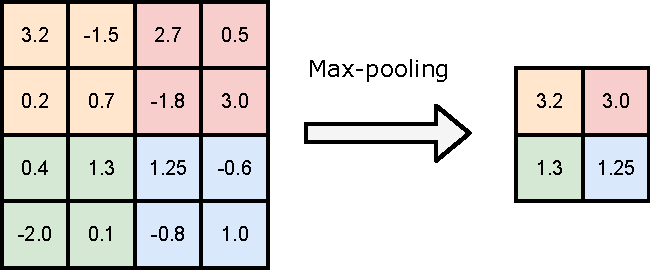
\includegraphics[width=0.5\textwidth]{images/max_pooling}
    \caption{Визуализация макс-пулинга 2x2 на изображении (4,4,1). Для нескольких каналов операция применяется независимо к каждому каналу.
}
    \label{fig:max_pooling}
\end{SCfigure}

Мы можем построить свёрточный «блок», объединив несколько свёрточных слоев с операцией макс-пулинга (см. Рисунок \ref{fig:cnn_blocks}):
%
$$
\text{ConvBlock}(X)= (\text{MaxPool} \circ \phi \circ \text{Conv}\circ\ldots\circ\phi\circ\text{Conv})(X)
$$
%
И более сложную сеть, объединив несколько таких блоков:
%
\begin{equation}
H = (\text{ConvBlock}\circ\text{ConvBlock}\circ\ldots\circ\text{ConvBlock})(X)
\label{eq:convolutive_backbone}
\end{equation}
%
Этот дизайн имеет большое количество гиперпараметров: выходные каналы каждого слоя, размер ядра каждого слоя и т.д. Обычно пространство поиска для дизайна резко сокращается путем введения некоторых упрощающих предположений. Например, дизайн VGG \cite{szegedy2015going} популяризировал идею сохранения постоянного размера фильтра в каждом слое (например, $k=3$), при сохранении постоянного количества каналов в каждом блоке и удвоении их между каждым блоком.

\begin{SCfigure}
    \centering
    \hspace{1em}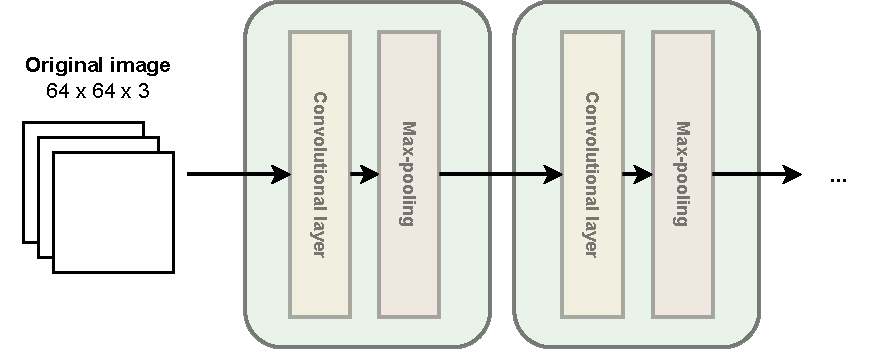
\includegraphics[width=0.6\textwidth]{images/CNN_blocks}
    \caption{Абстрагирование от «слоев» к «блокам» для упрощения проектирования дифференцируемых моделей.}
    \label{fig:cnn_blocks}
\end{SCfigure}

Альтернативный способ уменьшения размерности — это уменьшение выборки выхода свёрточного слоя: это называется \textbf{шагом} свёртки. Например, свёртка с шагом $1$ — это обычная свёртка, в то время как свёртка с шагом $2$ будет вычислять только один выходной пиксель на каждые $2$, свёртка с шагом $3$ будет вычислять один выход на каждые $3$ пикселя и так далее. Большие шаги и макс-пулинг также можно комбинировать в зависимости от того, как спроектирована вся модель.

\begin{supportbox}{Инвариантность и эквивариантность}
Неформально, если $T$ — это преобразование на $x$ из некоторого множества (например, все возможные сдвиги), мы говорим, что функция $f$ эквивариантна, если $f(Tx)=Tf(x)$, и инвариантна, если $f(Tx)=f(x)$. Пространство всех преобразований образует группу \cite{bronstein2017geometric}, и матрица, соответствующая конкретному преобразованию, называется \textbf{представлением} для этой группы. Свёртточные слои эквивариантны к трансляциям по своей конструкции, но можно найти и другие стратегии для более общих форм симметрий, такие как усреднение по элементам группы (\textbf{усреднение по фреймам}, \cite{puny2021frame}). Мы увидим другие типы эквивариантности слоев в Главе \ref{chap:gnns} и Главе \ref{chap:transformers}.
\end{supportbox}

\subsection{Проектирование полной модели}

Теперь мы можем завершить проектирование нашей модели. Объединив несколько свёрточных блоков, как в \eqref{eq:convolutive_backbone}, выход $H$ будет иметь форму $(h^\prime, w^\prime, c^\prime)$, где $w^\prime$ и $h^\prime$ зависят от количества операций макс-пулинга (или от шага свёрточных слоев), в то время как $c^\prime$ будет зависеть только от гиперпараметров последнего свёрточного слоя в последовательности. Обратите внимание, что каждый элемент $H_{ij}$ будет соответствовать «макро-области» на исходном изображении, например, если $h^\prime, w^\prime = 2$, $H_{11}$ будет соответствовать «верхнему левому» квадранту на исходном изображении. Мы можем устранить эту пространственную зависимость, выполнив заключительную операцию глобального пулинга перед классификацией. 

Полная модель, таким образом, может быть разложена на три основных компонента: серия свёрточных блоков, глобальный средний пулинг и заключительный блок для классификации.
%
\begin{align} 
H = (\text{ConvBlock}\circ\ldots\circ\text{ConvBlock})(X) \label{eq:conv_blocks} \\
\mathbf{h}= \frac{1}{h^\prime w^\prime}\sum_{i,j}H_{ij}  \label{eq:global_avg_pooling} \\
y=\text{MLP}(\mathbf{h}) \label{eq:classification_head}
\end{align}
%
где $\text{MLP}(\mathbf{h})$ — это общая последовательность полносвязных слоев (вместо глобального пулинга можно также использовать операцию сплющивания). Это прототипический пример СНС. См. Рисунок \ref{fig:cnn_architecture} для проработанного примера.

\begin{figure}
    \centering
    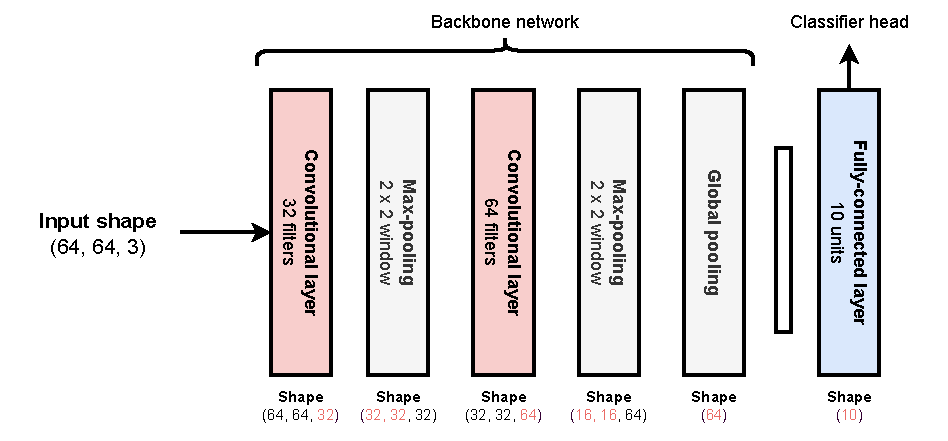
\includegraphics[width=0.9\textwidth]{images/CNN_architecture}
    \caption{Проработанный дизайн очень простой СНС для классификации изображений (предполагая 10 выходных классов). Мы показываем форму выхода для каждого слоя внизу. Операцию глобального пулинга можно заменить операцией сплющивания. Последнее (\textbf{скрытое}) представление перед классификационной головой очень полезно при дообучении крупномасштабных предварительно обученных моделей — это \textbf{вложение} изображения в смысле Раздела \ref{subsec:variants_supervised_learning}.}
    \label{fig:cnn_architecture}
\end{figure}

Этот дизайн имеет несколько интересных свойств, которые мы перечислим здесь:

\begin{enumerate}
\item Его можно обучать так же, как модели, описанные в Главе \ref{chap:linear_models} и Главе \ref{chap:fully_connected_models}. Например, для классификации мы можем обернуть выход в softmax и обучать, минимизируя кросс-энтропию. Те же правила обратного распространения ошибки, описанные в Главе \ref{chap:automatic_differentiation}, применяются и здесь.
\item Из-за операции глобального пулинга он не зависит от конкретного разрешения входа. Однако принято фиксировать это во время обучения и вывода, чтобы упростить мини-пакетирование (подробнее о входах переменной длины в следующей главе).
\item \eqref{eq:global_avg_pooling} можно рассматривать как блок «извлечения признаков», а \eqref{eq:classification_head} — как «классификационный блок». Эта интерпретация будет очень полезна, когда мы будем рассматривать трансферное обучение в следующем томе. Мы называем блок извлечения признаков \textbf{основой} модели, а классификационный блок — \textbf{головой} модели.
\end{enumerate}

\subsection*{Известные типы свёрток}

Мы завершаем главу, упомянув два примера свёрточных слоев, которые часто встречаются на практике. 

Во-первых, рассмотрим свёрточный слой с $k=0$, т.е. так называемую свёртку $1 \times 1$. Это соответствует обновлению вложения каждого пикселя взвешенной суммой его каналов, без учета всех остальных пикселей:
%
$$
H_{{\color{drawred}ij}z} = \sum_{t=1}^c W_{zt}X_{{\color{drawred}ij}t}
$$
%
Это полезная операция, например, для изменения размерности канала (мы увидим пример, когда будем иметь дело с остаточными соединениями в Главе \ref{chap:deep_cnns}). В этом случае параметры можно компактно представить матрицей $\mathbf{W} \sim (c^\prime, c)$. Это эквивалентно полносвязному слою, применяемому к каждому пикселю независимо.

Во-вторых, рассмотрим «ортогональный» вариант свёрток $1 \times 1$, в котором мы комбинируем пиксели в небольшом соседстве, но без учета всех каналов, кроме одного:
%
$$
H_{ij{\color{drawred}c}} = \sum_{i^\prime=1}^{2k+1}\sum_{j^\prime = 1}^{2k+1} W_{i^\prime, j^\prime,{\color{drawred}c}}X_{i^\prime +t(i),j^\prime+t(j),{\color{drawred}c}}
$$
%
где $t(\bullet)$ — это смещение, определенное в \eqref{eq:convolutive_offset}. В этом случае у нас есть весовая матрица 3-го ранга $W$ формы $(s, s, c)$, и каждый выходной канал $H_{:,:,c}$ обновляется, рассматривая только соответствующий входной канал $X_{:,:,c}$. Это называется \textbf{глубинной свёрткой}, и ее можно обобщить, рассматривая группы каналов, и в этом случае она называется \textbf{групповой свёрткой} (причем глубинная свёртка является крайним случаем размера группы, равного $1$).

Мы также можем комбинировать эти две идеи и иметь свёрточный блок, состоящий из чередующихся свёрток $1 \times 1$ (для смешивания каналов) и глубинных свёрток (для смешивания пикселей). Это называется \textbf{глубинно-разделимой} свёрткой и часто встречается в СНС, предназначенных для маломощных устройств \cite{howard2017mobilenets}. Обратите внимание, что в этом случае количество параметров для одного блока (по сравнению со стандартной свёрткой) уменьшается с $sscc^\prime$ до $ssc + cc^\prime$. Позже мы увидим, как эти разложения, где вход обрабатывается попеременно по отдельным осям, являются фундаментальными для других типов архитектур, таких как трансформеры, в Главе \ref{chap:transformers}.

\section*{От теории к практике}

\begin{wrapfigure}{r}{3.0cm}
\vspace{-3em}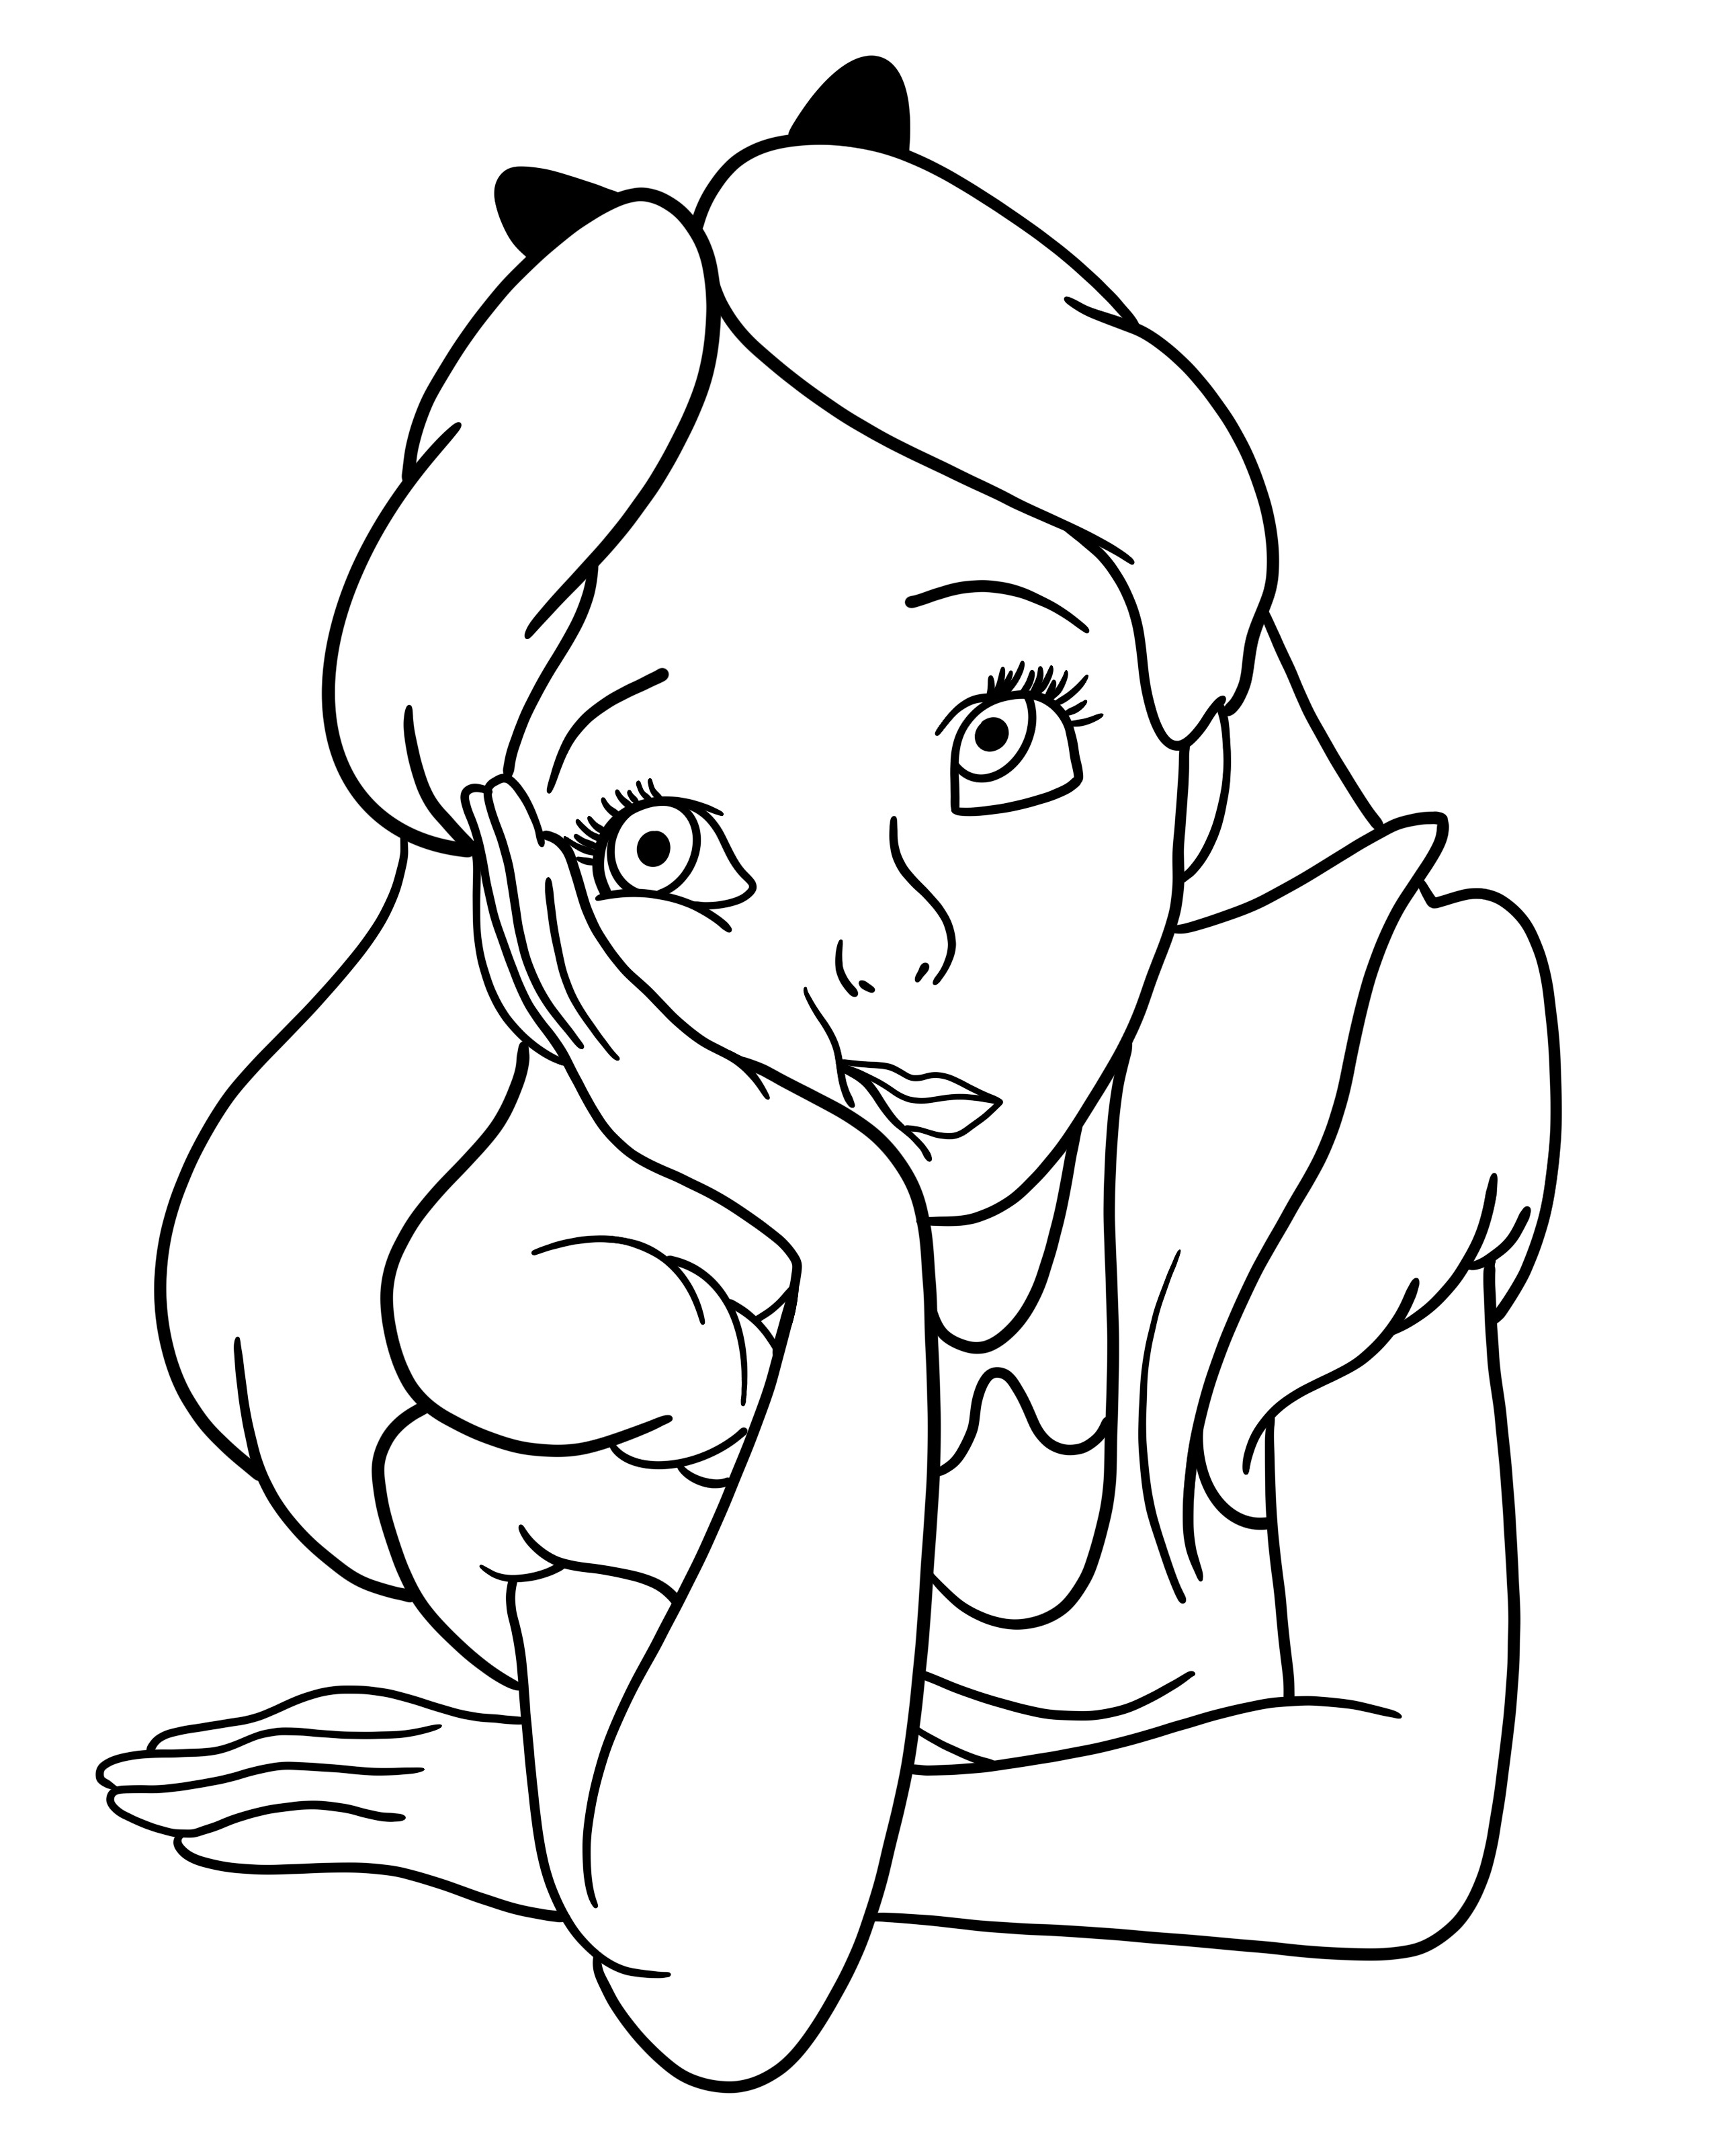
\includegraphics[width=3.0cm]{images/shutterstock_2075221579.jpg}
\vspace{-2em}
\end{wrapfigure}

Все слои, представленные в этой главе (свёртка, макс-пулинг), реализованы в модуле \mintinline{python}{torch.nn}. Библиотека torchvision предоставляет наборы данных и функции для загрузки изображений, а также интерфейс для применения преобразований к изображениям, который будет очень полезен в следующей главе.\footnote{\url{https://pytorch.org/vision/stable/transforms.html}} 

Прежде чем продолжить, я предлагаю вам проследить и перереализовать одно из многих онлайн-руководств по классификации изображений в torchvision, которое теперь должно быть относительно легко понять.\footnote{В качестве примера из официальной документации: \url{https://pytorch.org/tutorials/beginner/blitz/cifar10_tutorial.html}} Игрушечных наборов данных изображений предостаточно, включая MNIST (классификация цифр) и CIFAR-10 (общая классификация изображений). Сочетание загрузчика torchvision со слоями в Equinox позволяет воспроизвести то же руководство в JAX, например, \url{https://docs.kidger.site/equinox/examples/mnist/}.

Реализация свёртки с нуля также является интересным упражнением, сложность которого зависит от уровня абстракции. Одна из возможностей — использовать операции \texttt{fold}/\texttt{unfold} из PyTorch для извлечения патчей.\footnote{См., например: \url{https://github.com/loeweX/Custom-ConvLayers-Pytorch}} Готовые ядра для свёрток всегда будут значительно быстрее, что делает это чисто дидактическим упражнением.

Если у вас есть некоторый опыт в обработке сигналов, вы можете знать, что свёртку также можно реализовать как умножение, перейдя в частотную область. Это непрактично для маленьких ядер, которые мы обычно используем, но может быть полезно для очень больших (также известных как \textit{длинных}) свёрток, например, \url{https://github.com/fkodom/fft-conv-pytorch}. PyTorch также предоставляет дифференцируемое быстрое преобразование Фурье, которое вы можете использовать в качестве отправной точки.